\documentclass[parskip=full]{scrartcl}

\pdfoutput=1

\title{Increasing the Effectiveness of Active Learning:\\ 
	\LARGE{Introducing Artificial Data Generation in Active Learning for Land Use/Land Cover Classification}}
\author{
	Joao Fonseca\(^{1}\), Georgios Douzas\(^{1}\), Fernando Bacao\(^{1*}\) 
	\\
	\small{\(^{1}\)NOVA Information Management School, Universidade Nova de Lisboa}
	\\
	\small{*Corresponding Author}
	\\
	\\
	\small{Postal Address: NOVA Information Management School, Campus de Campolide, 1070-312 Lisboa, Portugal}
	\\
	\small{Telephone: +351 21 382 8610}
}

\usepackage{breakcites}
\usepackage{float}
\usepackage{graphicx}
\usepackage{subcaption}
\usepackage{geometry}
\geometry{
	a4paper,
	left=18mm,
	right=18mm,
	top=8mm,
}
\usepackage{amsmath}
\newcommand{\inlineeqnum}{\refstepcounter{equation}~\mbox{(\theequation)}}
\usepackage{enumitem}
\usepackage[ruled,vlined]{algorithm2e}
\usepackage{booktabs}
\usepackage{pgfplotstable}
\pgfplotsset{compat=1.14}
\usepackage{longtable}
\usepackage{tabu}
\usepackage{hyperref}
\date{}

\begin{document}

\maketitle

\begin{abstract}
	TODO TODO TODO TODO TODO TODO TODO TODO TODO TODO TODO TODO TODO TODO TODO TODO
	TODO TODO TODO TODO TODO TODO TODO TODO TODO TODO TODO TODO TODO TODO TODO TODO
	TODO TODO TODO TODO TODO TODO TODO TODO TODO TODO TODO TODO TODO TODO TODO TODO
	TODO TODO TODO TODO TODO TODO TODO TODO TODO TODO TODO TODO TODO TODO TODO TODO
	TODO TODO TODO TODO TODO TODO TODO TODO TODO TODO TODO TODO TODO TODO TODO TODO
	TODO TODO TODO TODO TODO TODO TODO TODO TODO TODO TODO TODO TODO TODO TODO TODO
	TODO TODO TODO TODO TODO TODO TODO TODO TODO TODO TODO TODO TODO TODO TODO TODO
\end{abstract}

\section{Introduction}~\label{sec:introduction}

The technological development of air and space borne sensors, as well as the increasing number of
remote sensing missions have allowed the continuous collection of large amounts of high quality
remotely sensed data. This data is often composed of multi and hyper spectral satellite imagery,
essential for numerous applications, such as Land Use/Land Cover (LULC) change detection, ecosystem
management~\cite{Nagai2020}, agricultural management~\cite{Huang2018}, water resource
management~\cite{Wang2018}, forest management, and urban monitoring~\cite{Khatami2016}. However,
updating a LULC map is still a challenging task~\cite{Gavade2019, Wulder2018}. They can be updated
using either one of the following strategies:

\begin{enumerate}
    \item Photo-interpreted. Consists of evaluating a patch's LULC class based on orthophoto and
        satellite image interpretation~\cite{costa2020introducing}. This method guarantees a decent
        level of accuracy, as it is dependent on the interpreter's expertise and human
        error. Typically, it is an expensive, time-consuming task that requires the expertise of a
        photo-interpreter. This task is also frequently applied to obtain ground-truth labels for
        training and/or validating Machine Learning (ML) algorithms for related
        tasks~\cite{vermote2020remote, COSTANTINO2020}. 
    \item Automated mapping. It is based on the usage of a ML method or a combination of methods in
        order to obtain an updated LULC map. The development of a reliable automated method is still
        a challenge among the ML and remote sensing community, since the efficacy of existing
        methods vary across applications and geographical areas~\cite{Gavade2019}. Typically, this
        method requires the existence of ground-truth data, which is frequently outdated or
        nonexistent for the required time frame~\cite{Nagai2020}. On the other hand, employing a ML
        method provides readily available and relatively inexpensive LULC maps. The increasing
        quality of state-of-the-art classification methods have motivated the application and
        adaptation of these methods in this domain~\cite{Maxwell2018}.
    \item Hybrid approaches. They employ photo-interpreted data to augment the training dataset and
        improve the quality of automated mapping~\cite{Ruzicka2020}. It attempts to accelerate the
        photo-interpretation process by selecting a smaller sample of the study area to be
        interpreted. The goal is to minimize the inaccuracies found in the LULC map by
        supplying high-quality ground-truth data to the automated method. The final
        (photo-interpreted) dataset consists of only the most informative samples, i.e., patches
        that are typically difficult to classify for a traditional automated mapping
        method~\cite{Liu2020}. 
\end{enumerate}

The latter method is best know as Active Learning (AL). It is especially useful whenever there is an
absence of ground-truth data and/or the mapping region does not contain updated LULC
maps~\cite{Su2020}. In a context of limited sample-collection budget, the collection of the most
informative samples capable of optimally increasing the classification accuracy of a LULC map is of
particular interest~\cite{Su2020}. AL attempts to minimize the human-computer interaction involved
in photo-interpretation by selecting the data points to include into the classification process.
These data points are selected based on an uncertainty measure and represent the points close to the
decision borders. Afterwards, they are passed on for photo-interpretation and added to the training
dataset, while the points with the lowest uncertainty values are ignored for photo-interpretation
and classification. This process is iterated until a convergence criterion is
reached~\cite{Pasolli2016}. 

The relevant work developed within AL is described in detail in Section~\ref{sec:al-sota}.
The research attempts to address some of the challenges found in AL, mainly inherited from
automated and photo-interpreted mapping: mapping inaccuracies and time consuming
human-computer interactions. 
Mapping inaccuracies have different sources:

\begin{enumerate}
    \item Human error. The involvement of photo-interpreters in the data labeling step carries an
        additional risk to the creation of LULC patches. The minimum mapping unit being considered,
        as well as the quality of the orthophotos and satellite images being used, are some of the
        factors that may lead to the overlooking of small-area LULC patches and label-noisy training
        data~\cite{Pelletier2017}.
    \item High-dimensional datasets. The amount of bands (i.e., features) present in multi and hyper
        spectral images introduce an increased level of complexity in the classification
        step~\cite{Stromann2020}. These datasets are often prone to the Hughes phenomenon, also
        known as the curse of dimensionality. 
    \item Class separability. Producing an LULC map considering classes with similar spectral
        signatures makes them difficult to separate~\cite{Alonso-Sarria2019}. A lower pixel
        resolution of the satellite images may also imply mixed-class pixels, which may lead to
        both lower class separability as well as higher risk of human error.
    \item Existence of rare land cover classes. The varying morphologies of different geographical
        regions naturally implies an uneven distribution of land cover classes~\cite{Feng2018}. This
        is particularly relevant in the context of AL:\@ the data selection method is based on a
        given uncertainty measure over data points whose class label is unknown. Consequently, AL's
        iterative process of data selection may disregard wrongly classified land cover areas
        belonging to a minority class.
\end{enumerate}

Research developed in the field of Active Learning typically focus on the reduction of human error
by minimizing the human interaction with the process through the development of more efficient
choosers and selection criteria within the generally accepted AL framework.  Concurrently, the
problem of rare land cover classes is rarely addressed. This is a frequent problem in the ML
community, known as the Imbalanced Learning problem.  This problem exists whenever there is an
uneven between-class distribution in the dataset~\cite{Chawla2004}. Specifically, most classifiers
are designed to optimize metrics such as overall accuracy, which are designed to work primarily with
balanced datasets. Consequently, these metrics tend to introduce a bias towards the majority class
by attributing an importance to each class proportional to its relative
frequency~\cite{Maxwell2018}. As an example, such a classifier could achieve an overall accuracy of
99\% on a binary dataset where the minority class represents 1\% of the overall dataset and still be
deemed useless. A number of methods have been developed to deal with this problem. They can be
categorized into three different types of approaches~\cite{Fernandez2013,Kaur2019}. Cost-sensitive
solutions perform changes to the cost matrix in the learning phase. Algorithmic level solutions
modify specific classifiers to reinforce learning on minority classes. Resampling solutions modify
the dataset by removing majority samples and/or generating artificial minority samples. The latter
is independent from the context and can be used alongside any classifier. We will focus on
artificial data generation techniques, presented in Section~\ref{sec:ovs-sota}.

In this paper, we propose a novel AL framework to address two limitations commonly found in the
literature: Minimize human-computer interaction and reduce the class imbalance bias. This is done
with the introduction of an additional component in the iterative AL procedure (the generator), used
to generate artificial data to both balance and augment the training dataset. The introduction of
this component is expected to reduce the number of iterations required until convergence of the
predictor's quality.

This paper is organized as follows: Section~\ref{sec:introduction} exposes the problem and its
context, Sections~\ref{sec:al-sota} and~\ref{sec:ovs-sota} describe the state of the art in AL and
Oversampling techniques, Section~\ref{sec:proposed-method} exposes the proposed method,
Section~\ref{sec:methodology} covers the datasets, evaluation metrics, ML classifiers and
experimental procedure, Section~\ref{sec:results} presents the results and statistical analyses and
Section~\ref{sec:conclusion} reports the conclusions drawn from our findings.

\section{Active Learning Approaches}~\label{sec:al-sota}

AL is used as the general definition of frameworks aiming to train a learning system in multiple
steps, where a set of new data points are chosen and added to the training dataset each
time~\cite{Ruzicka2020}. Typically, an AL framework is composed of 10 elements, out of which 4 are
datasets, 2 are queries or estimations regarding the target class labels and 4 are components
responsible for performing the tasks involved in AL~\cite{Sverchkov2017,Su2020,Ruzicka2020}:

\begin{enumerate}
    \item Data source. In the context of LULC classification, the data source is usually a
        hyper/multi-spectral image, a Synthetic-aperture radar (SAR) image, or a composite image.
    \item Unlabeled dataset. Consists of a sample of the original data source. It is used in
        combination with the chooser and the selection criterion to retrieve uncertainty estimates
        on each iteration.
    \item Initial training sample. It is a small sample of the unlabeled dataset, used to initiate
        the first AL iteration. The size of the initial training sample normally varies between no
        observations at all and 10\%~\cite{Li2013}.
    \item Augmented training dataset. This dataset is the concatenation of the labeled initial
        training sample along with the datasets labeled by the oracle in past iterations.
    \item Uncertainty map. The dataset containing the highest uncertainty points/patches to be
        labeled by the oracle.
    \item Oracle. An external entity to which the uncertainty map is presented to. The oracle is
        responsible for annotating unlabeled samples to be added to the augmented dataset. In remote
        sensing, the oracle is typically a photo-interpreter, as is the case in~\cite{li2020}. Some
        of the research also refers to the oracle as the \textit{supervisor}~\cite{Su2020,
        Shrivastava2021}.
    \item Chooser. Produces the class probabilities for each unlabeled sample. This is a classifier
        trained using the augmented dataset. It is used to estimate the class probabilities for each
        sample over the unlabeled dataset.
    \item Selection criterion. It quantifies the chooser's uncertainty level for each sample
        belonging to the unlabeled dataset. It is typically based on the class probabilities
        assigned by the chooser. In some situations, the chooser and the selection criterion are
        grouped together under the concept \textit{acquisition function}~\cite{Ruzicka2020} or
        \textit{query function}~\cite{Su2020}. Some of the literature refers to the selection
        criterion by using the concept \textit{sampling scheme}~\cite{Liu2020}.
    \item Predictor. The classifier used to infer the land cover classes for the final output map.
        Once a stopping criterion is met, the classifier is trained using the augmented dataset and
        the LULC classes are inferred from the data source.
    \item Prediction output. In the context of LULC classification, the prediction output is the
        estimated LULC map raster.
\end{enumerate}

Figure~\ref{fig:al_typical} schematizes the steps involved in a complete AL iteration. For a better
context within the remote sensing domain, the prediction output is identified as the LULC map. This
framework starts by collecting unlabeled data from the original data source. It is used to generate
a random initial training sample and is labeled by the oracle. In practical applications, the oracle
is frequently a group of photo-interpreters~\cite{Kottke2017}. The chooser is trained on the
resulting dataset and is used to predict the class probabilities on the unlabeled dataset. They are
fed into a selection criterion to estimate the prediction's uncertainty, out of which the samples
with the highest uncertainty will be selected. This calculation is motivated by the absence of
labels in the uncertainty dataset. Therefore, it is impossible to estimate the prediction's accuracy
in a real case scenario. The iteration is completed when the selected points are tagged by the
oracle and added to the training dataset (i.e., the augmented dataset). 

\begin{figure}[htb]
	\centering
	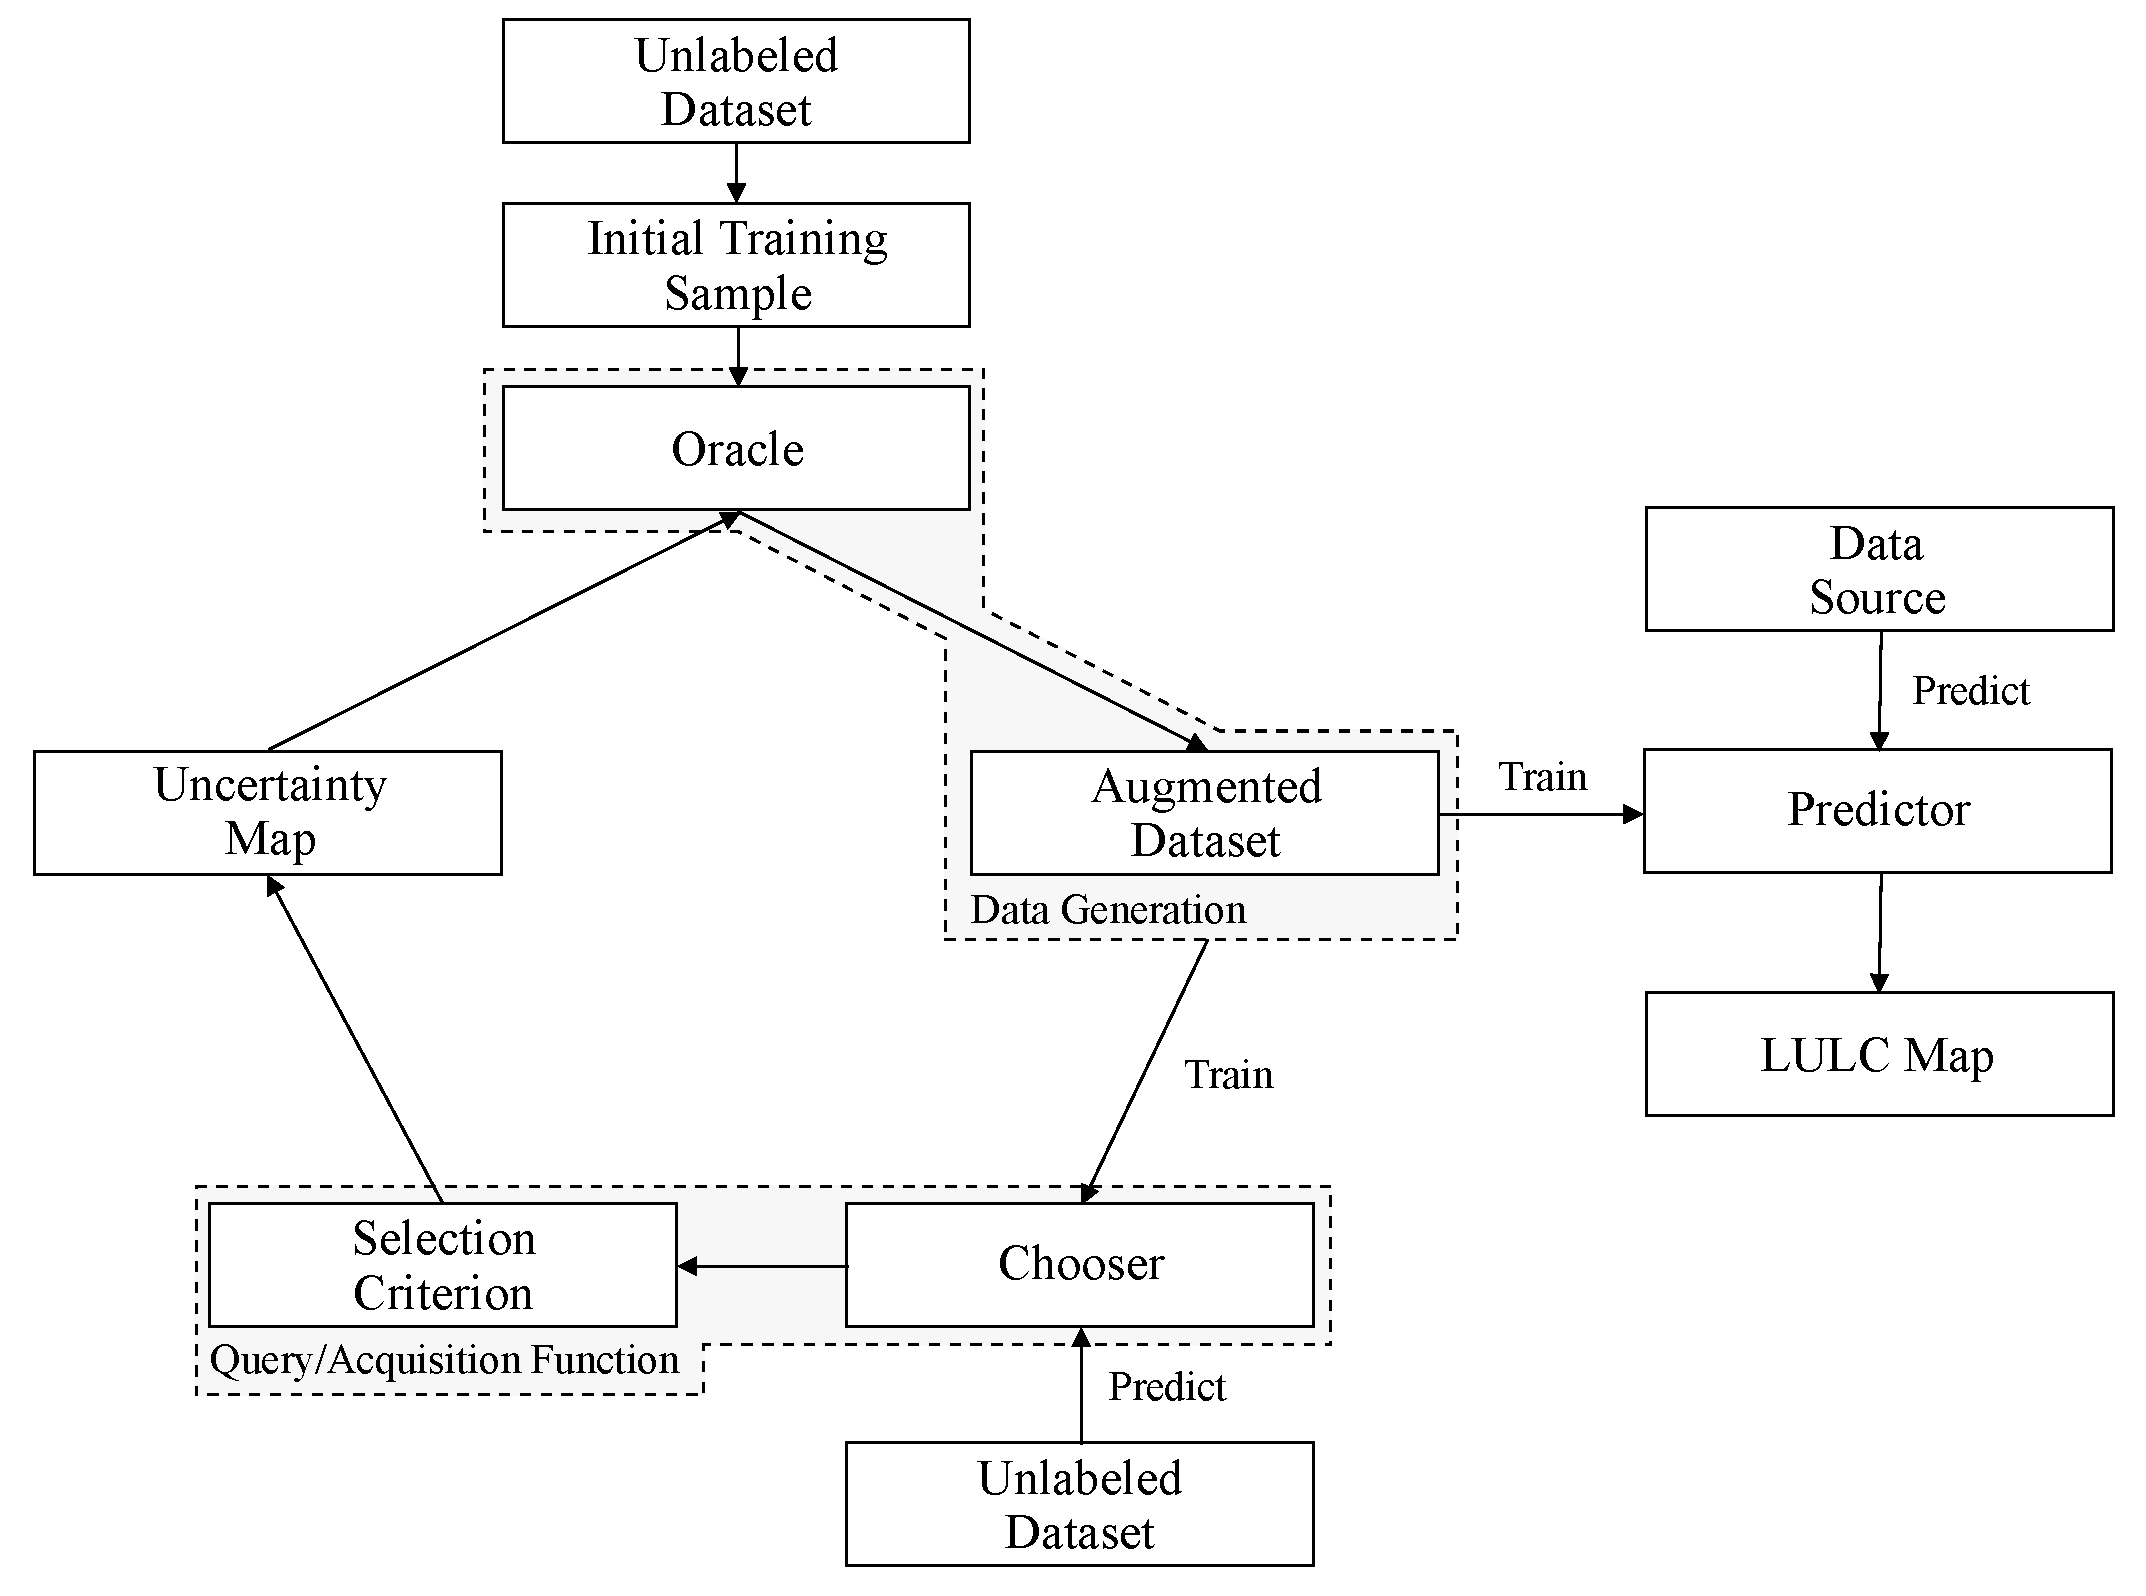
\includegraphics[width=.85\linewidth]{../analysis/al_typical}
	\caption{Typical AL framework.
    }~\label{fig:al_typical}
\end{figure}

Selecting an efficient selection criterion is particularly important to find the samples closest
to the decision border (i.e., samples difficult to classify)~\cite{Shrivastava2021}. Therefore, most
of AL related studies focus on the design of the query/acquisition function~\cite{Su2020}. There are
\textbf{X} main selection criteria

\subsection{Non-informed selection criteria}

Only one non-informed selection criterion was found. Random sampling selects unlabeled samples
without considering any external information produced by the chooser. Since the method for selecting
the unlabeled samples is random, this method disregards the usage of a chooser and is comparatively
worse than any other selection criterion. Although, random sampling is still a powerful baseline
method~\cite{Cawley2011}. Generally, different AL initializations return high performance
variability~\cite{Kottke2017}. When this happens, the analysis of the mean performances over multiple
repetitions is not of interest. Instead, it is preferable to do pairwise comparison of different
methods along with their corresponding variances. 

\subsection{Ensemble-based selection criteria}

Ensemble disagreement is based on the class predictions of a set of classifiers. The disagreement
between all the predictions for a given observation is a common measure for uncertainty, although
computationally inefficient~\cite{Ruzicka2020,Pasolli2016}. This method was implemented successfully
for complex applications like deep active learning~\cite{Ruzicka2020}.

Multiview~\cite{Muslea2006} consists on the training of multiple independent classifiers using
different views, which correspond to the selection of subsets of features or observations in the
dataset. Therefore, it can be seen as a bootstrap aggregation (bagging) ensemble disagreement
method. The set of classifications over a single observation is used to calculate the maximum
disagreement metric, given by the number of votes assigned to the most frequent
class~\cite{Shrivastava2021}. A lower value for this metric means a higher classification
uncertainty. Multiview-based maximum disagreement has been successfully applied to hyper-spectral
image classification in~\cite{Di2012} and~\cite{Zhou2014}.
% check whether the definition is 100% correct.

An adapted disagreement criterion for an ensemble of $k$-nearest neighbors has been proposed
in~\cite{Pasolli2016}. This method employs a $k$-nearest neighbors classifier and computes an
instance's classification uncertainty based on the neighbors' class frequency using the maximum
disagreement metric over varying values for $k$. As a result, this method is comparable to computing
the dominant class' score over a weighted $k$-nearest neighbors classifier. This method was also
used on a multimetric active learning framework~\cite{Zhang2016}.

Another relevant ensemble-based selection criterion is the binary random forest-based query
model~\cite{Su2020}. This method employs a one-versus-one ensemble method to demonstrate an
efficient data selection method using the estimated probability of each binary random forest and
determining the classification uncertainty based on the probabilities closest to 0.5 (i.e., the
least separable pair of classes are used to determine the uncertainty value). Although, this study
fails to compare the proposed method with other benchmark methods, such as random sampling.

\subsection{Entropy-based criteria}

A number of contributions have focused on entropy-based querying. The application of entropy is
common among active deep learning applications~\cite{Aghdam2019}, where the training of an ensemble
of classifiers is often too expensive. The measure of entropy is formulated as follows:

\begin{equation}
    H(x_i) = \sum_{\omega=1}^{N_i}{p(y_{i}^{*}=\omega|x_i)}\log_2[p(y_{i}^{*}=\omega|x_i)]
\end{equation}

The measurement of entropy $H$ is based on the observed probability $p(y_{i}^{*}=\omega|x_i)$ of
obtaining class $\omega$ as the predicted class label $y_{i}^{*}$, where $N_i$ is the number classes
predicted for observation $x_i$.

Entropy query-by-bagging (EQB), also defined as maximum entropy~\cite{Liu2020}, is an ensemble approach of
the entropy selection criterion, originally proposed in~\cite{Tuia2009}. This strategy uses the set
of predictions produced by the ensemble classifier to calculate those many entropy measurements.
The estimated uncertainty measure for one sample is given by the maximum entropy within that set.
EQB was observed to be an efficient selection criterion. Specifically, \cite{Shrivastava2021}
applied EQB on hyper-spectral remote sensing imagery using Support Vector Machines (SVM) and Extreme
Learning Machines (ELM) as choosers, achieving optimal results when combining EQB with ELM. This
method was also successful when applied alon




Query by bagging normalization~\cite{Copa2010}

\cite{Shrivastava2021}


- Margin Sampling
\cite{Shrivastava2021}
SVM specific, it's the distance of the point to the decision boundary

- Multiclass Level Uncertainty
\cite{Shrivastava2021}

- Breaking Ties 

- Mutual information

- Loss prediction~\cite{Yoo2019} 

Some of the literature fail to specify the strategy employed, although inferring it is generally
intuitive. For example,~\cite{Ertekin2007} successfully used AL to address the imbalanced learning
problem. They employed an ensemble of Support Vector Machines as the chooser and predictor to employ
the ensemble-based selection criterion.

Another frequent object of study is the chooser and predictor (which is often the same classifier).
% citation



% selection criteria

% maximum difference = margin sampling
% entropy
% model evaluations (agreement/disagreement rate)
% random sampling (used as a baseline method)

\section{Artificial Data Generation Approaches}~\label{sec:ovs-sota}

\subsection{Non-informed resampling methods}

\subsection{Heuristic methods}

\section{Proposed method}~\label{sec:proposed-method}

\begin{figure}[H]
	\centering
	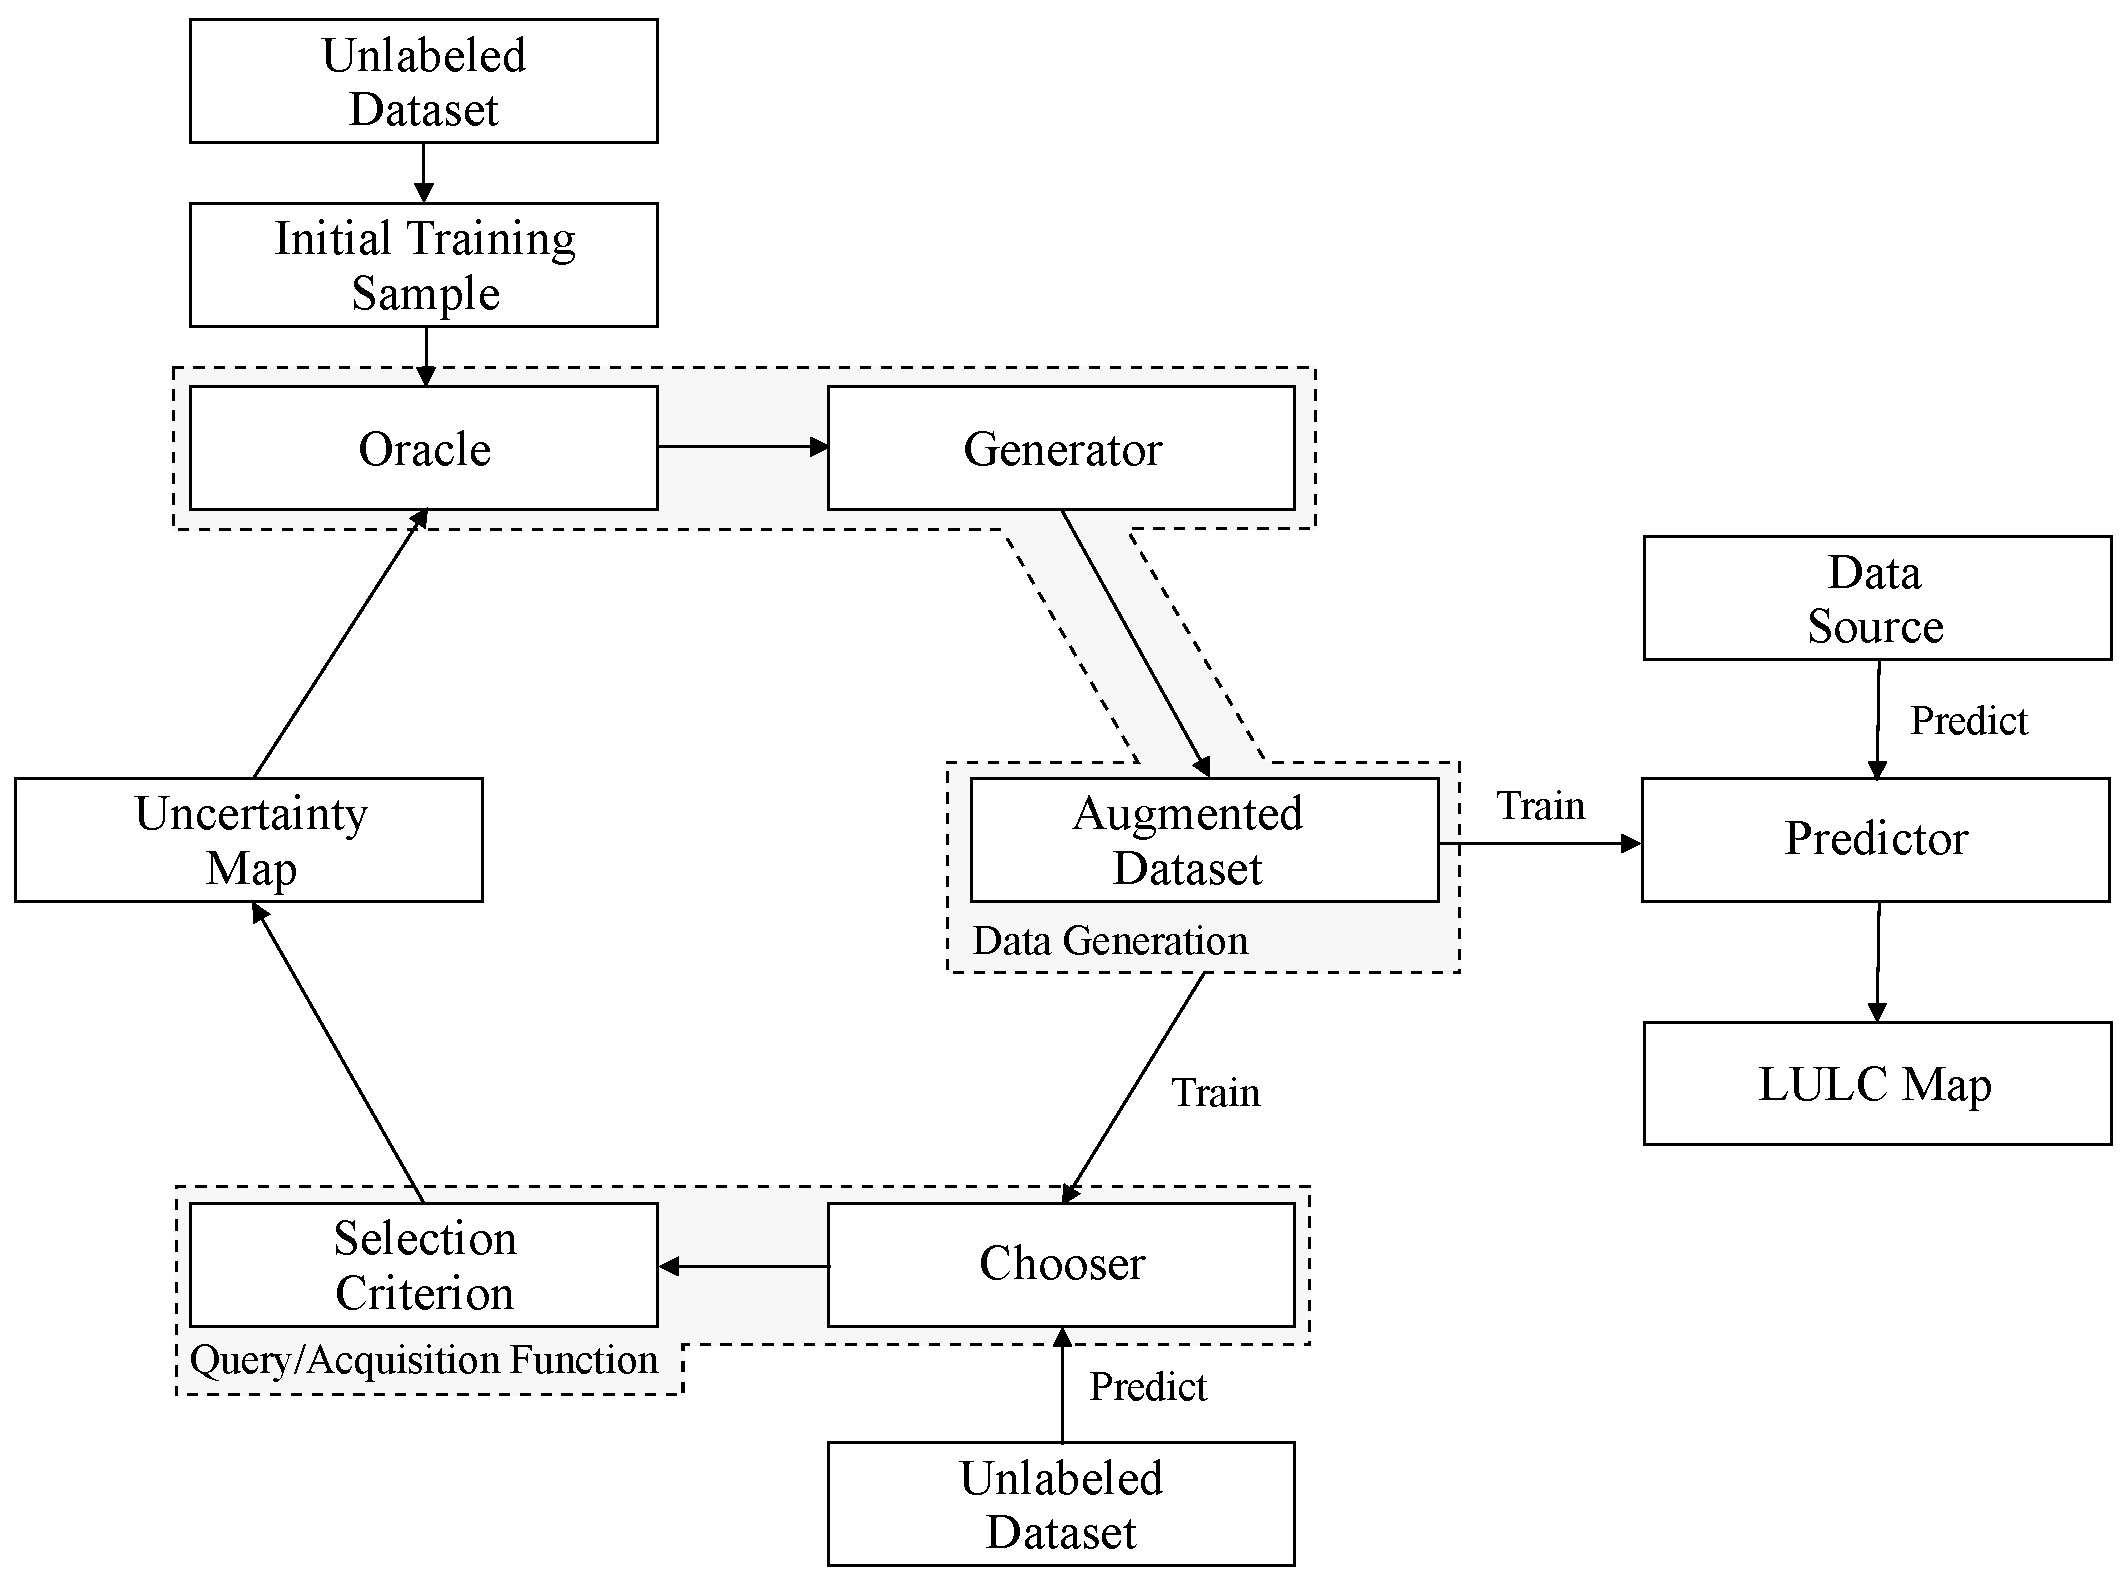
\includegraphics[width=.85\linewidth]{../analysis/al_new}
	\caption{Proposed AL framework.
    }~\label{fig:al_new}
\end{figure}

\section{Methodology}~\label{sec:methodology}

\subsection{Datasets}

\subsection{Evaluation Metrics}

\subsection{Machine Learning Algorithms}

\subsection{Experimental Procedure}

% source: http://arxiv.org/abs/1907.00038
A common practice in methodological evaluations is the implementation of an offline
experiment~\cite{Kagy2019}. It consists of using an existing set of labeled data as a proxy for the
population of unlabeled samples. Because the dataset is already fully labeled, the oracle's typical
annotation process involved in each iteration is done at zero cost.

% evaluation criteria

% AL with vs without oversampling
% AL with and without random oversampling
% AL vs fully labeled dataset

\subsection{Software Implementation}

\section{Results}~\label{sec:results}

\subsection{Statistical Analysis}

\section{Conclusion}~\label{sec:conclusion}

\bibliography{references}
\bibliographystyle{apalike}

\end{document}
